\documentclass{article}
\usepackage{amsmath}
\usepackage{graphicx}
\usepackage{url}
\usepackage{placeins}
\graphicspath{{images/}}

% Margins
\topmargin=-0.45in
\evensidemargin=0in
\oddsidemargin=0in
\textwidth=6.5in
\textheight=9.0in
\headsep=0.25in

%Title Info
\title{\vspace{-2cm}Particle Filters} %remove the extra spacing at the top
\author{Alex Pan and Alec Kosik}
\date{} %blank the date

\begin{document}
\maketitle

% --------------------- Abstract ---------------------
\begin{abstract}
Particle Filters allow us to model non-linear and non-Gaussian distributions through Monte Carlo methods. We first discuss HMM, and then discuss a recursive formulation of the distribution of $p(x_t|y_{1:t})$ and how this leads well to an algorithmic approach. Finally, we investigate Kalman Filters, Importance Sampling, and SIR. We discuss the motivations for and relevant problems with each approach.
\end{abstract}

% --------------------- Motivation ---------------------
\section{Introduction}

Imagine that we have some outside information about a system and that we can generate observations which are dependent on the state of the system. However, the actual state of the system is hidden from us. How can we go about finding the hidden state of the system using our observations? It turns out we can approximate the hidden state through a process called \textbf{particle filtering}.

To give a toy example of this, imagine that we have a robot in a room. We know the layout of the room, but we do not know the position of our robot. However, the robot is able to take some sort of measurements with a sensor, for example its distance to walls. Using the sensor data and our existing information about the layout of the room, we use particle filtering to make predictions about where we could be in the room.

We will begin by formally defining the problem setting and then deriving particle filtering algorithms.

% --------------------- Preliminaries ---------------------
\section{Hidden Markov Models}

A \textbf{Hidden Markov Model} (HMM) is defined as a Markov process with states that cannot be observed, but gives outputs that are dependent on the hidden state of the system. If we let the random variable $X_i$ represent the $i$-th state of the system, and the random variable $Y_i$ represent the $i$-th output of the system, we have:
\begin{equation}
X_1 \sim \mu (x_1) \textnormal{ and } X_n|(X_{n-1}=x_{n-1}) \sim f(x_n|x_{n-1})
\end{equation}
\begin{equation}
Y_n|(X_n = x_n) \sim g(y_n|x_n)
\end{equation}
where $X_1$ is defined by some initial conditions $\mu(x_1)$. Note how $f$ obeys the Markov property, so the current state $x_n$ is dependent only on the previous state $x_{n-1}$. Also note that $g$ shows that the current observation $y_n$ is only dependent on the current state $x_n$.

Let $x_{1:t}$ represent the ordered n-tuple of hidden states $(x_1,\dots,x_n)$ where $x_i$ is the $i$-th hidden state. Similarly, let $y_{1:t}$ represent the ordered n-tuple of observations $(y_1,\dots,y_n)$. There are a few important distributions that follow directly from our HMM setting.
% this derivation is confusing (1) because of the switch from p to f and (2) because of the application of bayes rule to get derive line 2. i think it would be better to just give the equation in 1 line and explain where it comes from in prose.
\begin{equation} \label{p(x_{1:t})}
\begin{split}
p(x_{1:t})
&= p(x_1)p(x_2|x_1)p(x_3|x_2,x_1)\dots p(x_n|x_{n-1},\dots,x_1)\\
&= p(x_1)p(x_2|x_1)p(x_3|x_2)\dots p(x_n|x_{n-1})\\
&=\mu(x_1)\prod_{i=2}^{n} f(x_i|x_{i-1})\\
\end{split}
\end{equation}

\begin{equation} \label{p(y_{1:t}|x_{1:t})}
\begin{split}
p(y_{1:t}|x_{1:t})
&= p(y_1|x_{1:t})p(y_2|x_{1:t},y_1)(y_3|x_{1:t},y_2,y_1)\dots (y_n|x_{1:t},y_{n-1},\dots,y_1)\\
&= p(y_1|x_1)p(y_2|x_2)\dots (y_n|x_n)\\
&= \prod_{i=1}^{n} g(y_i|x_i)\\
\end{split}
\end{equation}


% --------------------- Setting up the problem ---------------------
\section{Problem Setup}
\subsection{General Goals}
There are a few different uses of the particle filtering method. We could model the distribution $p(x_{1:t}|y_{1:t})$, the distribution $p(x_n|y_{1:t})$, or even the expected value of functions defined on these distributions. Here, our main goal is to use our observations to determine the hidden state of the system. That is, we want to figure out $p(x_{n}|y_{1:t})$. This is recognizable as the marginal of $p(x_{1:t}|y_{1:t})$.

\begin{equation}
p(x_{n}|y_{1:t}) = \int p(x_{1:t}|y_{1:t}) dx_{1:n-1}
\end{equation}

Setting our goal as a marginal of $p(x_{1:t}|y_{1:t})$ is helpful because we can refactor the full conditional distribution to see how it comes from our prior distributions derived in \eqref{p(x_{1:t})} and \eqref{p(y_{1:t}|x_{1:t})}. Refactoring and using our initial HMM conditions, we can show:

\begin{equation} \label{pfiltereq}
\begin{split}
p(x_{1:t}|y_{1:t}) &= \frac{p(x_{1:t},y_{1:t})}{p(y_{1:t})}\\
&= \frac{p(x_{1:t}) p(y_{1:t}|x_{1:t})}{p(y_{1:t})}\\
&= \frac{p(x_{1:t}) p(y_{1:t}|x_{1:t})}{\int p(x_{1:t},y_{1:t}) dx_{1:t}}\\
&= \frac{\mu(x_1)\prod_{i=2}^{n} f(x_1|x_{i-1})\prod_{i=1}^{n} g(y_i|x_i)}{\int \mu(x_1)\prod_{i=2}^{n} f(x_1|x_{i-1})\prod_{i=1}^{n} g(y_i|x_i) dx_{1:t}}
\end{split}
\end{equation}

\noindent
Thus,

\begin{equation} \label{monster}
p(x_n|y_{1:t}) = \int \frac{\mu(x_1)\prod_{i=2}^{n} f(x_1|x_{i-1})\prod_{i=1}^{n} g(y_i|x_i)}{\int \mu(x_1)\prod_{i=2}^{n} f(x_1|x_{i-1})\prod_{i=1}^{n} g(y_i|x_i) dx_{1:t}} dx_{1:n-1}
\end{equation}

This looks really messy, but it's helpful to see that this is just integration of functions we already know: $f$ and $g$. Depending on whether these integrals are analytically tractable, which is not always the case, we can obtain the goal distribution $p(x_n|y_{1:t})$ from \eqref{monster}.

%In other words, we already have all the information we need to arrive at the answer.

\subsection{A Recursive Formulation}
In cases where the integrals in \eqref{monster} are tractable, we can evaluate them. However, it would be really inefficient if we had to evaluate \eqref{monster} at every time step. Instead, we can formulate this recursively and see how some of the values carry through. This recursiveness is described in two parts: the marginal prediction equation and the marginal update equation.

\subsubsection{Marginal Prediction Equation}
We now show how to derive the prediction equation:
\begin{equation} \label{mpredict}
p(x_t|y_{0:t-1}) = \int f(x_t|x_{t-1})p(x_{t-1}|y_{0:t-1}) dx_{t-1}
\end{equation}
\begin{align*}
\intertext{If we approach this as a marginal by integrating out $x_{t-1}$ we normally would formulate this as:}
p(x_t|y_{0:t-1}) &= \int p(x_{t-1:t}|y_{0:t-1}) dx_{t-1}\\
&= \int p(x_t|x_{t-1},y_{0:t-1})p(x_{t-1}|y_{0:t-1}) dx_{t-1}\\
\intertext{We can make use of the Markov property to see:}
p(x_t|x_{t-1},y_{0:t-1}) &= p(x_t|x_{t-1}) = f(x_t|x_{t-1})\\
\end{align*}

\subsubsection{Marginal Update Equation}
\begin{equation} \label{mupdate}
p(x_t|y_{0:t}) = \frac{p(x_t|y_{0:t-1})p(y_t|x_t)}{p(y_t|y_{0:t-1})}
\end{equation}

The derivation will be broken into 2 parts. First, we will show that \eqref{mupdate} holds iff $p(x_t,y_{0:t}) = p(x_t,y_{0:t-1})p(y_t|x_t)$ holds. Then we will show that $p(x_t,y_{0:t}) = p(x_t,y_{0:t-1})p(y_t|x_t)$. We start by applying Bayes' rule to the left side of \eqref{mupdate} and then moving the denominator to the right side:

\begin{align*}
p(x_t,y_{0:t}) &= \frac{p(x_t|y_{0:t})p(y_t|x_t)}{p(y_t|y_{0:t-1})}p(y_{0:t}) \\
\intertext{Applying Bayes' rule to $p(x_t|y_{0:t})$:}
&= \frac{p(x_t,y_{0:t})p(y_t|x_t)}{p(y_t|y_{0:t-1})p(y_{0:t-1})}p(y_{0:t}) \\
&= \frac{p(x_t,y_{0:t})p(y_t|x_t)}{p(y_{0:t})}p(y_{0:t}) \\
&= p(x_t,y_{0:t})p(y_t|x_t)
\end{align*}

\noindent
Second, we show $p(x_t,y_{0:t}) = p(x_t,y_{0:t-1})p(y_t|x_t)$. Let's start by refactoring the right-side.
\begin{align*}
p(x_t,y_{0:t-1})p(y_t|x_t) &= p(x_t|y_{0:t-1})p(y_{0:t-1})\frac{p(x_t,y_t)}{p(x_t)}\\
&= p(x_t|y_{0:t-1})p(y_{0:t-1})\frac{p(x_t|y_t)p(y_t)}{p(x_t)}\\
\intertext{Using the fact that: $p(x|yz) =$ {\Large $\frac{p(y)p(z)}{p(yz)}\frac{p(x|y)p(x|z)}{p(x)}$}
  Let: $x=x_t, y=y_{0:t-1}, z = y_t$}
\intertext{We can now see that:  $p(x_t|y_{0:t-1},y_t) =$ {\Large $\frac{p(y_{0:t-1})p(y_t)}{p(y_{0:t-1},y_t)}\frac{p(x_t|y_{0:t-1})p(x_t|y_t)}{p(x_t)}$}}
\intertext{Thus,}
p(x_t|y_{0:t-1})p(y_{0:t-1})\frac{p(x_t|y_t)p(y_t)}{p(x_t)} &= p(x_t|y_{0:t})p(y_{0:t})\\
&= p(x_t,y_{0:t})\\
\end{align*}

The equations \eqref{mpredict} and \eqref{mupdate} give us what we will call the \textit{marginal prediction} and \textit{marginal update} steps respectively. They also make clear an algorithmic approach: by repeating these steps at each time $t$, we can find
$p(x_t|y_{0:t})$ for any $t$, from our initial state up to our $n$-th state. This is also far more computationally efficient because we can save time by using information we already have from the previous iteration, instead of trying to perform a large integration at every single step. Unfortunately, when the integral in the prediction step is not solvable analytically we cannot recursively calculate it. In the Subsection \ref{sec:kalman} we will briefly describe a situation in which we can recursively calculate the marginal prediction and marginal update steps. Then in Subsection \ref{sec:pfiltering} we will describe the more general particle filtering method for use in cases where the marginal prediction and marginal update equations are not recursively calculable.

% --------------------- Kalman Filter ---------------------
\subsection{Kalman Filter} \label{sec:kalman}

Setting different kinds of constraints on the problem leads to different kinds of solutions. It turns out that when $p(x_{t-1},y_{0:t-1})$ is Gaussian, we can show that $p(x_{t},y_{0:t})$ is Gaussian provided that $f$ and $g$ are linear functions on their inputs. In cases when these conditions hold, we can use the \textbf{Kalman Filter} to find $p(x_{t},y_{0:t})$.

Essentially the Kalman Filter reformulates everything in terms of matrices since $f$ and $g$ are linear. An important thing to note is that the Kalman Filter typically extends our problem setting to include noise. That is to say, our transition and observation distributions both have noise parameters. In a physical setting, this might look something like the wind blowing on the robot while it moves, which might affect its location as it moves, and uncertainty in our sensor data, which is what we would expect in any real life measurement.

We can then reformulate $x_k$ and $y_k$ as a system of matrix equations, and also show that \eqref{mpredict} and \eqref{mupdate} turn out to be Gaussian distributions. From there, we can derive another set of equations that give us the Kalman Filter, but we won't go through a statement or proof of these equations because some of the linear algebra goes outside the scope of this discussion.

\subsection{Particle Filtering} \label{sec:pfiltering}
When the integral in the marginal prediction step is not analytically calculable, our recursive formulation of the marginal prediction and marginal update steps is not computationally recursive. That is, although \eqref{mpredict} and \eqref{mupdate} look recursive, they are not because the integral in \eqref{mpredict} does not decompose. In such cases, we will turn back to equation \eqref{pfiltereq} and simulate that distribution, rewritten as:

\begin{equation}
\begin{split}
p(x_{1:t}|y_{1:t}) &= \frac{p(x_{1:t}) p(y_{1:t}|x_{1:t})}{\int p(x_{1:t},y_{1:t}) dx_{1:t}}\\
&= \frac{\mu(x_1)\prod_{i=2}^{n} f(x_1|x_{i-1})\prod_{i=1}^{n} g(y_i|x_i)}{p(y_{1:t})} \\
&= p(x_{1:n-1},y_{1:n-1}) \frac{f(x_n|x_{n-1})g(y_n|x_n)}{p(y_n|y_{1:n-1})} \\
&\propto p(x_{1:n-1},y_{1:n-1}) f(x_n|x_{n-1})g(y_n|x_n)
\end{split}
\end{equation}

\noindent
This equation is easily calculable because we always know $f$ and $g$ and we know $p(x_{1:n-1},y_{1:n-1})$ recursively. We do not know $p(y_n|y_{1:n-1})$, but it can be ignored since we only care about the probability of a given path of states $x_{1:t}$ relative to the probability of other states---hence the $\propto$. In this scenario we have the following prediction and update steps\footnote{These prediction and update steps are more common in the particle filtering literature since the marginal prediction and marginal update steps are computationally expensive in non-linear, non-gaussian contexts}:

\begin{equation} \label{predict}
\textnormal{Prediction step:  }
p(x_{1:t}|y_{1:t-1})= f(x_t|x_{t-1}) p(x_{1:t-1}|y_{1:t-1})
\end{equation}

\begin{equation} \label{update}
\textnormal{Update step:  }
p(x_{1:t}|y_{1:t})\propto g(y_t|x_t)p(x_{1:t}|y_{1:t-1})
\end{equation}

Let's assess our current situation. We want to find the distribution for $p(x_t|y_{1:t})$. We found a calculable equation for $p(x_{1:t}|y_{1:t})$ and noticed that our goal is just a marginal of this. We tried integrating $p(x_{1:t}|y_{1:t})$ over $x_{1:t-1}$ to get our marginal but our best expression of this integral is only recursively calculable under certain constraints. When $p(x_{1:t}|y_{1:t})$ does not abide by these constraints we have no analytical solution and thus turn to a \textit{simulation} method called particle filtering. In the next section we will explicate a monte carlo method that will help us model $p(x_{1:t}|y_{1:t})$ by recursively simulating the distributions of \eqref{predict} and \eqref{update} at each time step.

\section{Monte Carlo Methods}

In general, \textit{not just in the particle filtering case}, we can model any distribution $\pi(x_{1:n})$ by sampling from $\pi$: $x_{1:n}^{(i)} \sim \pi(x_{1:n})$ for $i=1,\dots,N$, and then assigning each sample a probability of $1/N$. For example, if $x_{1:n}^{(i)} = x_{1:n}^{(j)} = (x_1,\dots,x_n)$ then the probability that $X_{1:n} = (x_1,\dots,x_n)$ is $2/N$. Thus we can represent our simulated model of $\pi$ by:

\begin{equation}
\widehat{\pi}(x_{1:n}) = \begin{cases}
1/N \quad \text{at} \ x_{1:n}^{(1)} \\
\vdots \\
1/N \quad \text{at} \ x_{1:n}^{(N)} \\
\end{cases}
\end{equation}

We can then move towards an approximation of \eqref{predict} and \eqref{update} by sampling from our transition distribution at each time step $x_{t}^{(i)} \sim f(x_t|x_{t-1})$ for $i = 1,\dots,N$. Using these samples, we build an approximate distribution for the transition distribution where each particle $i$ has probability equal $1/N$. For now, we are only concerned with the probability of $x_t$ based on the last state $x_{t-1}$.
%Notice that our sample $x_{t}^{(i)}$ comes from the transition probability; thus we must combine it with the tuple of past states $(x_{1:t-1}^{(i)},x_{t}^{(i)})$.

\begin{equation}
\widehat{f}(x_t|x_{t-1}) = \begin{cases}
1/N \quad \text{at} \ x_{t}^{(1)} \\
\vdots \\
1/N \quad \text{at} \ x_{t}^{(N)} \\
\end{cases}
\end{equation}

As is, this method does not seem very helpful since we are modelling a distribution that we can sample from so, presumably, we already know the distribution analytically. In the next section we'll see why this simulation technique is important.


% --------------------- SIS ---------------------
\section{Importance Sampling \& Sequential Importance Sampling}
In this section we will develop the basic but not widely used method of particle filtering. In doing so, we deal with the full posterior $p(x_{1:t}|y_{1:t})$. However, simulating this distribution is the same as simulating our goal distribution, the marginal of the full posterior, $p(x_t|y_{1:t})$. The only difference is that the full posterior will be a $t$-dimensional model while our goal will just be a model of the $t$-th dimension.

\subsection{Importance Sampling}
Importance sampling allows us to sample from a proposal distribution $p(x_{1:n})$, one we know e.g. a uniform or gaussian, and then weight samples from this proposal distribution to match the target distribution $t(x_{1:n})$ that we want to sample from. At first, this may sound like a trick---if we know the weight (difference) between the target and proposal, how could we not know the target---but if we consider our weight to be something like our function $g$, IS begins to make sense. Assuming we can approximate the prediction step by assigning each sample $x_{1:t}^{(i)}$ a probability $w_{1:t-1}^{(i)}$, which we will show in the next subsection, we can then approximate the update step as follows:

\begin{equation}
\widehat{p}(x_{1:t}|y_{1:t}) = \begin{cases}
w_{1:t-1}^{(1)}\frac{g(y_k|x_k^{(1)})}{\sum_{j=1}^N g(y_k|x_k^{(j)})} \quad \text{at} \ x_{1:t}^{(1)} \\
\vdots \\
w_{1:t-1}^{(N)}\frac{g(y_k|x_k^{(N)})}{\sum_{j=1}^N g(y_k|x_k^{(j)})} \quad \text{at} \ x_{1:t}^{(N)} \\
\end{cases}
\end{equation}

\subsection{Sequential Importance Sampling}
Our first particle filtering algorithm follows easily from the last two sections. We need to approximate the prediction and update distributions; we have already shown the prediction step. For each time step $t$ we estimate the update distribution:

\begin{equation}
\widehat{p}(x_{1:t}|y_{1:t-1}) = \begin{cases}
w_{1:t-1}^{(1)} \quad \text{at} \ x_{1:t}^{(1)} \\
\vdots \\
w_{1:t-1}^{(N)} \quad \text{at} \ x_{1:t}^{(N)} \\
\end{cases}
\end{equation}

\noindent
where $w_{1:t-1}^{(i)}$ are the normalized weights up to time $t$ defined as:

\begin{equation}
w_{1:t-1}^{(i)} = \prod_{k=1}^{t-1} \frac{g(y_k|x_k^{(i)})}{\sum_{j=1}^N g(y_k|x_k^{(j)})}
\end{equation}

\subsubsection{SIS Algorithm}
Simulating a particle $i$ up to time $t$, we are given a previous path $x_{1:t-1}^{(i)}$, weighted according to $w_{1:t-1}^{(i)}$. We then draw a current state $x_{t}^{(i)}$ from the transition distribution and add it to the current path $x_{1:t} = (x_{1:t-1}^{(i)},x_t^{(i)})$. This completes the prediction step. To update, we multiply the probability of $x_{1:t} = x_{1:t}^{(i)}$, written $p(x_{1:t}|y_{1:t-1}) = w_{1:t-1}^{(i)}$, by $\frac{g(y_t|x_t)}{\sum_{i=1}^N g(y_k|x_k^{(i)})}$.

\begin{enumerate}
\item \textit{Initialization:}
\item[] For $i=1,\dots N$:
\begin{itemize}
\item[] Sample $x_0^{(i)} \sim \mu(x_0)$
\item[] Assign weights $\widetilde{w}_0^{(i)} = g(y_0|x_0^{(i)})$
\item[] Normalize weights $w_0^{(i)} = \frac{\widetilde{w}_0^{(i)}}{\sum_{i=1}^{n} \widetilde{w}_0^{(i)}}$
\end{itemize}
\item \textit{Importance Sampling:}
\item[] For $t=1,\dots,T$:
\begin{itemize}
\item[] Sample $x_t^{(i)} \sim f(x_t|x_{t-1}^{i})$
\item[] Assign weights $\widetilde{w}_t^{(i)} = g(y_t|x_t^{(i)})$
\item[] Normalize weights $w_t^{(i)} = \frac{\widetilde{w}_t^{(i)}}{\sum_{i=1}^{n} \widetilde{w}_t^{(i)}}$
\end{itemize}
\item Return $\{x_T^{(i)},w_T^{(i)}\}_{i=1}^N$
\end{enumerate}

SIS is almost never used because of something called the ``degeneracy problem''. It does however, lay the groundwork for a widely used algorithm called SIR which we will discuss in the next section.

% --------------------- Degeneracy Problem ---------------------
\subsection{Degeneracy Problem}
When we are sampling from our reweighted distribution, it is possible that certain points are assigned very low weight. In future iterations, this is likely to compound, making their weights essentially negligible. This manifests as a handful of points having nearly all the weight while the rest of our points have ``degenerated''. This is a problem because our distribution essentially is now defined by just a few of the original points we started with, which is not enough to get an accurate representation of our target distribution.


% --------------------- Bootstrap/SIR ---------------------
\section{Bootstrap (SIR)}
We can effectively solve the degeneracy problem by resampling. After each iteration $t>0$ we will resample all $N$ particles from the weighted distribution defined in the previous time step. Thus particles with low-to-negligible weights at $t$ will have a low probability of persisting to $t+1$. See Figure \ref{fig:sir} for a visualization of this process.

\subsection{Bootstrap Algorithm}
\begin{enumerate}
\item \textit{Initialization:}
\item[] For $i=1,\dots N$:
\begin{itemize}
\item[] Sample $x_0^{(i)} \sim \mu(x_0)$
\item[] Assign weights $\widetilde{w}_0^{(i)} = g(y_0|x_0^{(i)})$
\item[] Normalize weights $w_0^{(i)} = \frac{\widetilde{w}_0^{(i)}}{\sum_{i=1}^{n} \widetilde{w}_0^{(i)}}$
\end{itemize}
\item \textit{Importance Sampling:}
\item[] For $t=1,\dots,T$:
\begin{itemize}
\item[] Sample $x_t^{(i)} \sim f(x_t|\widetilde{x}_{t-1}^{i})$
\item[] Assign weights $\widetilde{w}_t^{(i)} = g(y_t|x_t^{(i)})$
\item[] Normalize weights $w_t^{(i)} = \frac{\widetilde{w}_t^{(i)}}{\sum_{i=1}^{n} \widetilde{w}_t^{(i)}}$
\item[] Resample $\widetilde{x}_t^{(i)}$ from $x_t^{(i)}$ according to the weight distribution with replacement.
\end{itemize}
\item Return $\{x_T^{(i)},w_T^{(i)}\}_{i=1}^N$
\end{enumerate}

\begin{figure}
\centering
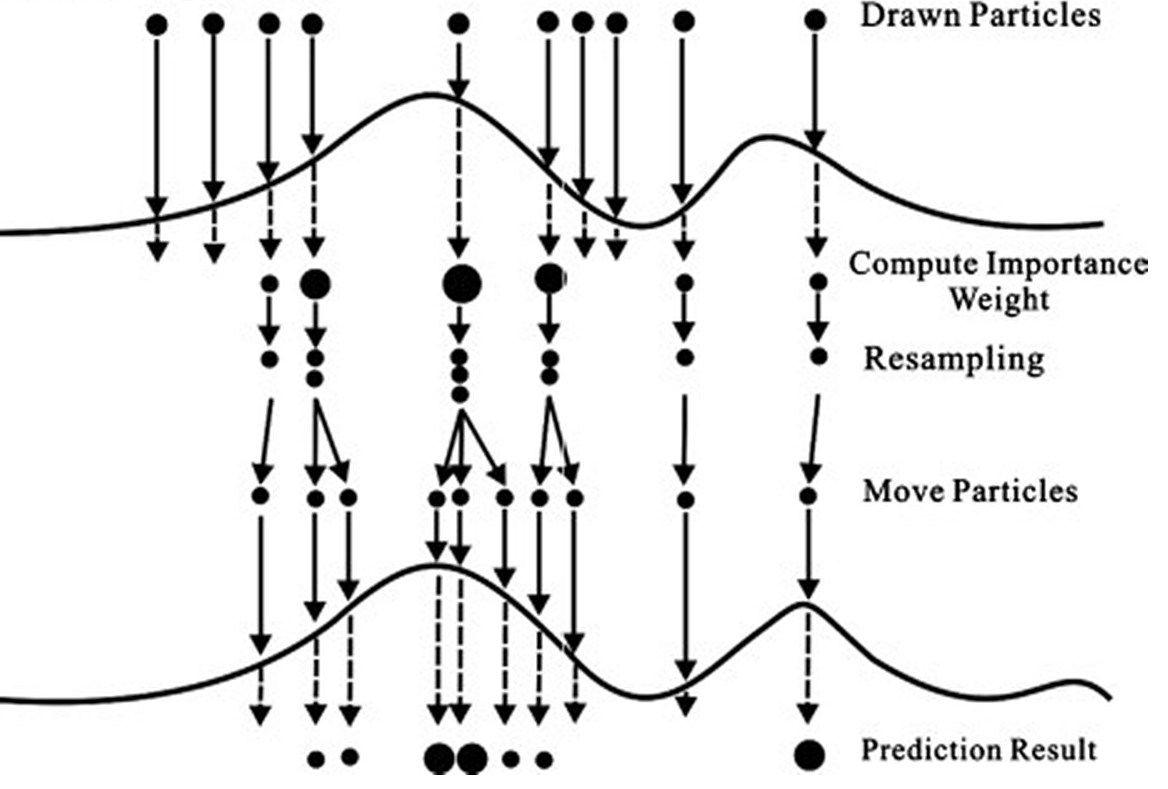
\includegraphics[scale=.25]{sir}
\caption{The SIR algorithm, adopted from \cite{sirfig}.}
\label{fig:sir}
\end{figure}

\subsection{Sampling Impoverishment Problem}
While this addresses the degeneracy problem, it turns out that resampling has it's own issue which we call the ``sampling impoverishment problem''. This comes about because our higher weighted points are more likely to be drawn multiple times. Instead of having many low-weight points spread out across the state-space---in the case of SIS and the degeneracy problem---we will have lots of evenly-weighted points concentrated around areas where high-weight points originally occurred. Intuitively, the degeneracy problem leaves you with a diverse scattering of point masses with a few ill-defined peaks while the sampling impoverishment problem leaves you with \textit{only} well defined peaks. There are methods that address both of these issues but they require fancy sounding things like the ``Epanechnikov Kernel'', which our outside the scope of our discussion. It turns out that SIR is generally good enough and is the algorithm that people generally use.

\FloatBarrier
\section{Conclusion}



% --------------------- Some equations!!! ---------------------

% \section{Lots of equations we'll use:}
% \begin{equation}
% \textnormal{Prior: }
% p(x_{1:t}) = \mu(x_1)\prod_{i=2}^{n} f(x_1|x_{i-1})
% \end{equation}

% \begin{equation}
% \textnormal{Conditional of Y: }
% p(y_{1:t}|x_{1:t}) = \prod_{i=1}^{n} g(y_i|x_i)
% \end{equation}

% \begin{equation}
% \textnormal{Conditional of X: }
% p(x_{1:t}|y_{1:t}) = \frac{p(x_{1:t},y_{1:t})}{p(y_{1:t})}
% \end{equation}

% \begin{equation}
% \textnormal{Joint: }
% p(x_{1:t},y_{1:t}) = p(x_{1:t}) p(y_{1:t}|x_{1:t})
% \end{equation}

% \begin{equation}
% \textnormal{Marginal: }
% p(y_{1:t}) = \int p(x_{1:t},y_{1:t}) dx_{1:t}
% \end{equation}

% \begin{equation}
% \textnormal{We have: }
% \{p(x_{1:t}|y_{1:t})\}_{n>0}
% \textnormal{ and }
% \{p(y_{1:t})\}_{n>0}
% \end{equation}

% \begin{equation}
% \textnormal{Want to find: }
% \{p(x_n|y_{1:t})\}_{n>0}
% \end{equation}

% \begin{equation}
% \textnormal{Reformulate the joint: }
% p(x_{1:t},y_{1:t}) = p(x_{1:n-1},y_{1:n-1}) f(x_n|x_{n-1}) g(y_n|x_n)
% \end{equation}

% \begin{equation}
% \begin{split}
% p(x_{1:t},y_{1:t}) &= p(x_{1:t}) p(y_{1:t}|x_{1:t})\\
% p(x_{1:t}) &= \mu(x_1)\prod_{i=2}^{n} f(x_1|x_{i-1})
% = (\mu(x_1)\prod_{i=2}^{n-1} f(x_1|x_{i-1})) f(x_n|x_{n-1})
% = p(x_{1:n-1} (x_n|x_{n-1}))\\
% p(y_{1:t}|x_{1:t}) &= \prod_{i=1}^{n} g(y_i|x_i)
% = (\prod_{i=1}^{n-1} g(y_i|x_i)) g(y_n|x_n)
% = p(y_{1:n-1}|x_{1:n-1}) g(y_n|x_n)\\
% p(y_{1:n-1}|x_{1:n-1}) &= \frac{p(x_{1:n-1},y_{1:n-1})}{p(y_{1:n-1})}\\
% p(x_{1:t},y_{1:t}) &= p(x_{1:n-1} (x_n|x_{n-1})) \frac{p(x_{1:n-1},y_{1:n-1})}{p(y_{1:n-1})} g(y_n|x_n)
% = p(x_{1:n-1},y_{1:n-1}) f(x_n|x_{n-1}) g(y_n|x_n)
% \end{split}
% \end{equation}

% \begin{equation}
% \textnormal{Reformulate the conditional of X: }
% p(x_{1:t}|y_{1:t}) = p(x_{1:n-1}|y_{1:n-1})\frac{f(x_n|x_{n-1}) g(y_n|x_n)}{p(y_n|y_{1:n-1})}
% \end{equation}

% \begin{equation}
% \begin{split}
% p(x_{1:t}|y_{1:t}) &= \frac{p(x_{1:t},y_{1:t})}{p(y_{1:t})}\\
% p(x_{1:t},y_{1:t}) &= p(x_{1:n-1},y_{1:n-1}) f(x_n|x_{n-1}) g(y_n|x_n)\\
% p(x_{1:n-1},y_{1:n-1}) &= p(y_{1:n-1}) p(x_{1:n-1}|y_{1:n-1})\\
% p(y_{1:n-1}) &= \frac{p(y_{1:n-1},y_n)}{p(y_n|y_{1:n-1})} = \frac{p(y_{1:t})}{p(y_n|y_{1:n-1})}\\
% p(x_{1:t}|y_{1:t}) &= \frac{1}{p(y_{1:t})}\frac{p(y_{1:t})}{p(y_n|y_{1:n-1})} p(x_{1:n-1}|y_{1:n-1}) f(x_n|x_{n-1}) g(y_n|x_n)\\
% &= p(x_{1:n-1}|y_{1:n-1})\frac{f(x_n|x_{n-1}) g(y_n|x_n)}{p(y_n|y_{1:n-1})}\\
% \end{split}
% \end{equation}

% \begin{equation}
% \pi_n(x_{1:t})=p(x_{1:t}|y_{1:t}) = \frac{p(x_{1:t},y_{1:t})}{p(y_{1:t})}
% \end{equation}

% \begin{equation}
% \hat{\pi}_n(x_{1:t})=\frac{1}{N}\sum_{i=1}^{N}\delta_{X_{1:t}^i}(x_{1:t})
% \end{equation}

% \begin{equation}
% \hat{\pi}_n(x_k)=\frac{1}{N}\sum_{i=1}^{N}\delta_{X_k^i}(x_k)
% \end{equation}

\newpage
\nocite{*}
\bibliography{Report}
\bibliographystyle{ieeetr}

\end{document}
